\section*{15th August}

\begin{itemize}
  \item received replacement external soundcard as the initial one was DoA (guess for\$3 dollars can't really complain). No problems using the bcm2835 kernel module. The following steps enable the card at init \url{http://www.linuxcircle.com/2013/05/08/raspberry-pi-microphone-setup-with-usb-sound-card/}.
  \item I increased the gain to +11db , otherwise a bit too quite for lecture recording.
  \item Encountered a lot of noise during recording which seems to be a biproduct of lack of shielding/circuit isolation on the Pi. Moving the device to a usb hub seems to have improved things though still sounds like clipping at the top end. Will keep trying.
  \item Lastly, finally got around to expanding the available root partition space with parted.. now have additional 13gig for sound storage. Instructions found here \url{http://www.raspberrypi.org/phpBB3/viewtopic.php?f=51&t=45265}
  \item Updated the test script to run 2 servos connected via the gpio pins, using software controls
prototype setup of 2 servos
\end{itemize}


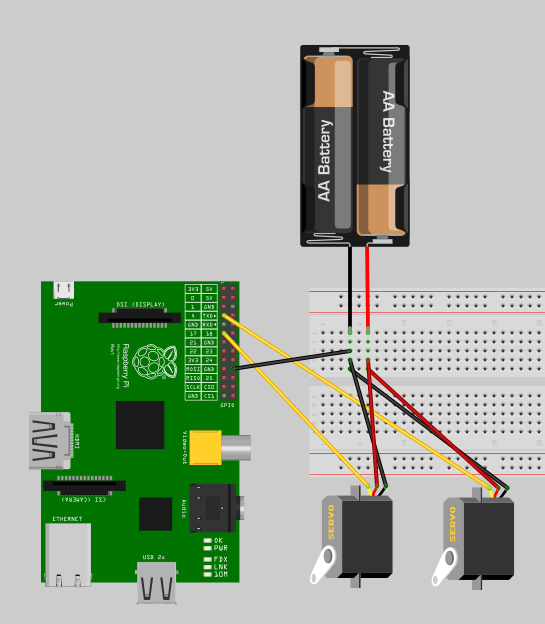
\includegraphics[width=\textwidth]{graphs/proto2.png}

\section*{18th August}

\begin{itemize}
  \item Completed assembling the usb servo controller and added pin connectors to power block and mechanical switch
  \item Tested out the PIR sensor, sample scripts uploaded including one with a on/off switch activation
  \item Got the pololu servo controller working over the USB virtual serial port, starting working on easing using the speed control... not sure if would use it though
\end{itemize}



\section*{19th August}

\begin{itemize}
  \item Put together a script for communicating with the Pololu servo over the USB serial port. Setting acceleration param does easing automatically which is pretty handy if we are going to do video recording at the same time as record.
  \item Still looking for a suitable base plate to attach to the Y servo bracket... a bit worried of whether the plastic gearing I have on X servo can handle the extra weight... may have to pick up a large metal gear from a hobby store if it starts to slip once the mic and camera are mounted on it.
  \item Starting to work on networking 2 RPis and whats an efficient (read: basic + lowest overhead) coms channel we can use for issues commands over.
\end{itemize}



\section*{30th September}

\begin{itemize}
  \item Creating a systemd service to launch the server (master) daemon...
    \begin{itemize}
      \item groupadd osp \# create a new group
      \item useradd -r -g osp osp \# create a system account osp in the new group
      \item chown osp:osp /usr/local/bin/osp\_server \# set ownership of the daemon
      \item add the service script (in src dir) to /etc/systemd/system/
      \item systemctl daemon-reload \# reloads the available services descriptions
      \item systemctl start osp-project.service \# to start the service straight away
      \item systemctl enable osp-project.service \# get the service to start at boot-time
    \end{itemize}
  \item Added a wireless interface to connect to backup router for maintenance config (network-wireless.service in src dir). Like before, systemctl daemon-reload/enable ...

\end{itemize}

